\documentclass[journal]{IEEEtran}

%\usepackage[retainorgcmds]{IEEEtrantools}
%\usepackage{bibentry}
\usepackage{xcolor,soul,framed} %,caption

\colorlet{shadecolor}{yellow}
% \usepackage{color,soul}
\usepackage[pdftex]{graphicx}
\graphicspath{{../pdf/}{../jpeg/}}
\DeclareGraphicsExtensions{.pdf,.jpeg,.png}

\usepackage[cmex10]{amsmath}
%Mathabx do not work on ScribTex => Removed
%\usepackage{mathabx}
\usepackage{array}
\usepackage{mdwmath}
\usepackage{mdwtab}
\usepackage{eqparbox}
\usepackage{url}


% ----------------------------------------------

% Definitions of languages: ------------
\usepackage{listings}
\lstdefinestyle{cStyle}{
  basicstyle=\scriptsize,
  breakatwhitespace=false,
  breaklines=true,
  captionpos=b,
  keepspaces=true,
  numbersep=5pt,
  showspaces=false,
  gobble=4,
  tabsize=4,
  showstringspaces=false,
  showtabs=false,
}
\renewcommand*{\lstlistingname}{Code}

% ----------------------------------------------




% \hyphenation{op-tical net-works semi-conduc-tor}

%\bstctlcite{IEEE:BSTcontrol}


%=== TITLE & AUTHORS ===========================================================
\begin{document}
\bstctlcite{IEEEexample:BSTcontrol}
    \title{Imitation Learning with Keras}
  \author{Carlos~Matheus~Barros~da~Silva,~
  \IEEEmembership{Computer Engineering Bachelor Student of ITA}
  \\Prof. Marcos~Ricardo~Omena~de~Albuquerque~Máximo}

% The paper headers
\markboth{INSTITUTO TECNOLÓGICO DE AERONÁUTICA, May~2019
}{Reinforcement Learning}

% ==============================================================================
\maketitle



% === ABSTRACT =================================================================
% ==============================================================================
\begin{abstract}

This paper evaluates the core concepts of the behind the Reinforcement Learning
theory on the environment of the Markov Decision Process (MDP).

It was observed how policy iteration and value itaration works and how they are
affected by the probability of correctly executing the chosen action factor
($\alpha$) and the discount factor($\gamma$).

It was observed that for a deterministic world ($\gamma = 1$ and $\alpha = 1$),
the learning is sensibly slower, which means that was required much more iterations
in order to the value converge when compared to a little decrease on $\gamma$ and
$\alpha$ ($\gamma = 0.98$ and $\alpha = 0.8$).

% === KEYWORDS =================================================================
% ==============================================================================
\begin{IEEEkeywords}
    Reinforcement Learning, policy, states
\end{IEEEkeywords}
\end{abstract}

\IEEEpeerreviewmaketitle
% ==============================================================================
% ==============================================================================
% ==============================================================================


% === I. INTRODUCTION ==========================================================
% ==============================================================================
\section{Introduction}

\IEEEPARstart{R}{e}inforcement learning (RL) is an area of machine learning
concerned with how software agents ought to take actions in an environment so
as to maximize some notion of cumulative reward. Reinforcement learning is one
of three basic machine learning paradigms, alongside supervised learning
and unsupervised learning.

It differs from supervised learning in that labelled input/output pairs need
not be presented, and sub-optimal actions need not be explicitly corrected.
Instead the focus is finding a balance between exploration (of uncharted
territory) and exploitation (of current knowledge).

The environment is typically formulated as a Markov decision process (MDP),
as many reinforcement learning algorithms for this context utilize dynamic
programming techniques. The main difference between the classical dynamic
programming methods and reinforcement learning algorithms is that the latter
do not assume knowledge of an exact mathematical model of the MDP and they
target large MDPs where exact methods become infeasible.

% ==========================================================================
\section{Neural Network Implementation}

The implementation was based on the file \textit{imitatino learning}. The essence of the implementation is shown in Code \ref{code:imitation}.

\lstinputlisting[
    language=python,
    caption={Code of \textit{imitatino learning}},
    label={code:imitation},
    style=cStyle,
    firstline=53,
    lastline=84
]{./../code/imitation_learning.py}

\section{Neural Network Analysis}

\subsection{Keras' Neural Network Analysis without regularization}

In this analysis was used two test functions: \textit{sum greater than} and \textit{xor}. This initial analysis is not using regularization.

The Keras' Neural Network performed regular on \textit{sum greater than} function. On the graphs represented by the images from Image \ref{img:greater_cost_no_reg} to Image \ref{img:greater_classification_no_reg}. It is possible to verify that the result is overfitted on the Image \ref{img:greater_classification_no_reg} and the convergence is not so fast on the Image \ref{img:greater_cost_no_reg}.

\begin{figure}
  \begin{center}
  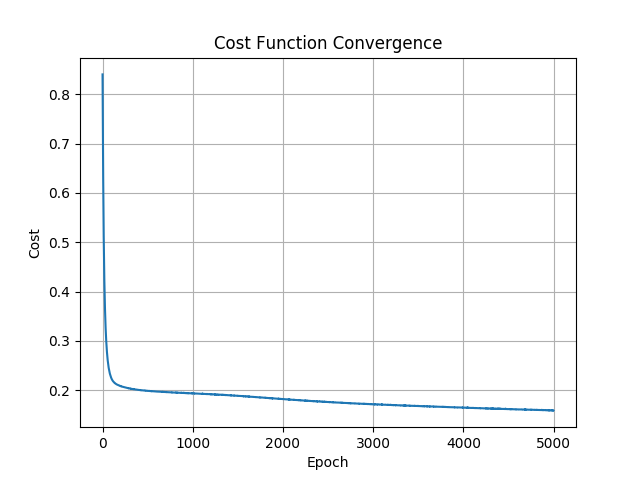
\includegraphics[width=2.8in]{./../code/sgz_result/convergence_sgz_l0_0.png}
  \caption{Convergence of cost function on greater than function test case, when it is not using regularization.}
  \label{img:greater_cost_no_reg}
  \end{center}
\end{figure}

\begin{figure}
  \begin{center}
  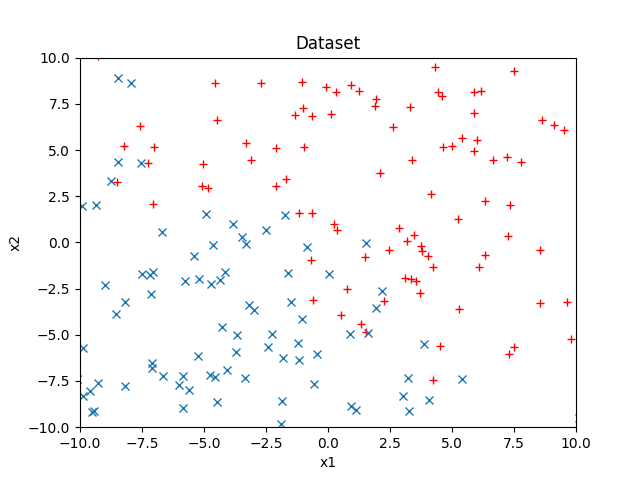
\includegraphics[width=2.8in]{./../code/sgz_result/dataset_sgz_l0_0.png}
  \caption{Dataset of greater than function.}
  \label{img:greater_data_set}
  \end{center}
\end{figure}

\begin{figure}
    \begin{center}
    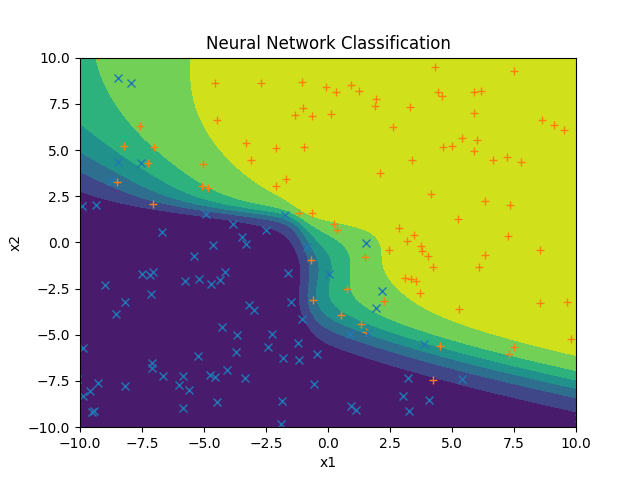
\includegraphics[width=2.8in]{./../code/sgz_result/nn_classification_sgz_l0_0.png}
    \caption{Neural Network Classification on greater than function, when it is not using regularization.}
    \label{img:greater_classification_no_reg}
    \end{center}
\end{figure}

The Neural Network performed regular on \textit{xor} function. On the graphs represented by the images from Image \ref{img:xor_cost_no_reg} to Image \ref{img:xor_classification_no_reg}. It is also possible to see that in this case, it also heaped some overfit causing some distortion and leading to some mistakes on the data set on the graph represented by the Image \ref{img:xor_classification_no_reg}.

\begin{figure}
  \begin{center}
  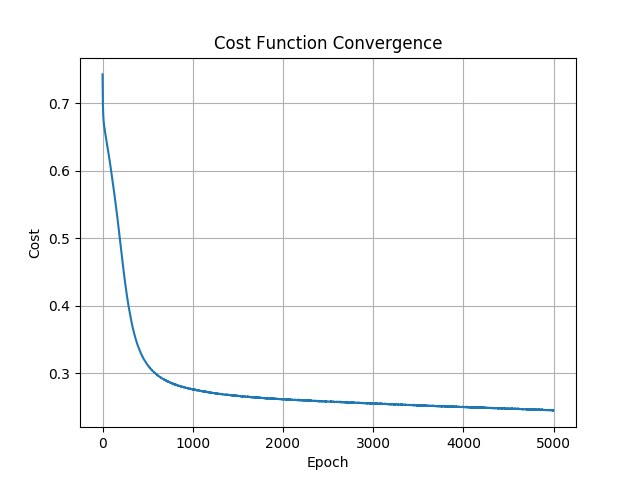
\includegraphics[width=2.8in]{./../code/xor_result/convergence_xor_l0_0.png}
  \caption{Convergence of cost function on xor function test case, when it is not using regularization.}
  \label{img:xor_cost_no_reg}
  \end{center}
\end{figure}

\begin{figure}
  \begin{center}
  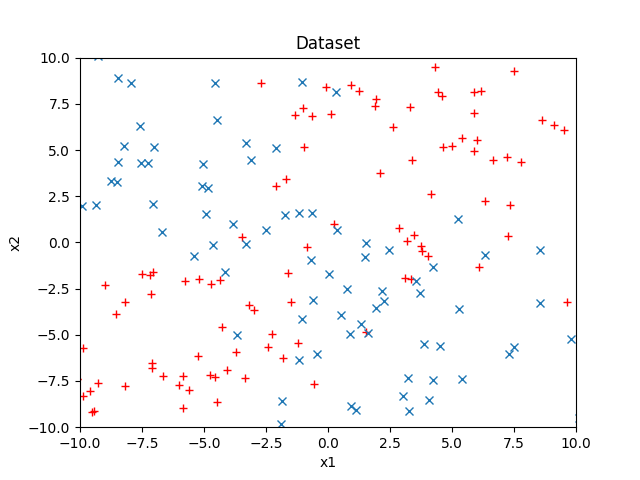
\includegraphics[width=2.8in]{./../code/xor_result/dataset_xor_l0_0.png}
  \caption{Dataset of xor function.}
  \label{img:xor_data_set}
  \end{center}
\end{figure}

\begin{figure}
    \begin{center}
    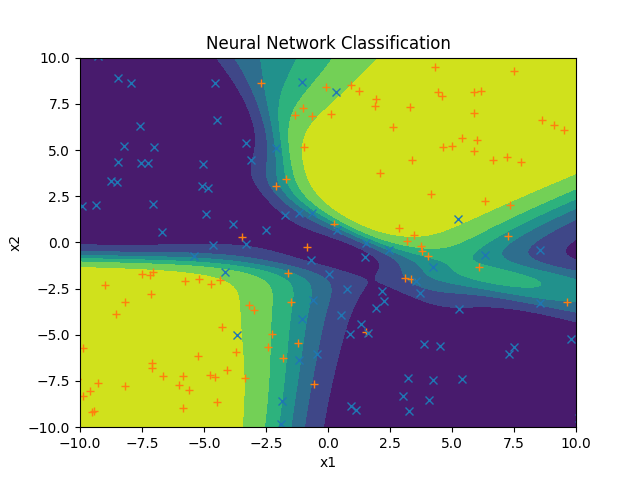
\includegraphics[width=2.8in]{./../code/xor_result/nn_classification_xor_l0_0.png}
    \caption{Neural Network Classification on xor function, when it is not using regularization.}
    \label{img:xor_classification_no_reg}
    \end{center}
\end{figure}

\subsection{Keras' Neural Network Analysis without regularization}

In this analysis was used the same two test functions: \textit{sum greater than} and \textit{xor}. But now using regularization $\lambda_{l_2} = 0.002$.

The Keras' Neural Network performed well on \textit{sum greater than} function. On the graphs represented by the images from Image \ref{img:greater_cost_reg} to Image \ref{img:greater_classification_reg}. It is possible to verify that the result now is much less overfitted on the Image \ref{img:greater_classification_reg}, it is much softer, and the convergence is now faster on the Image \ref{img:greater_cost_reg}.

\begin{figure}
  \begin{center}
  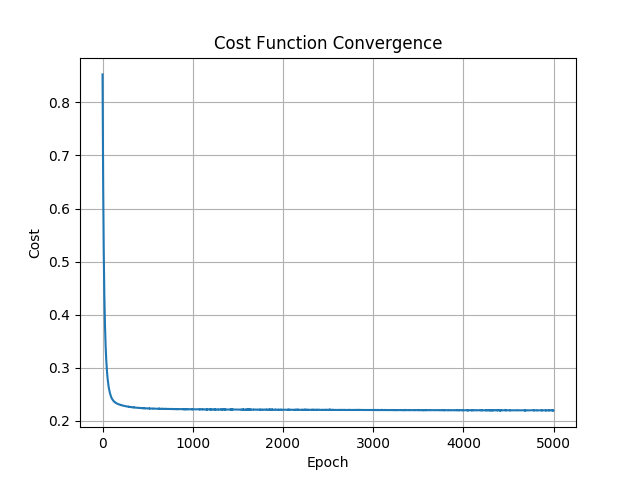
\includegraphics[width=2.8in]{./../code/sgz_result/convergence_sgz_l0_002.png}
  \caption{Convergence of cost function on greater than function test case, when it is using regularization.}
  \label{img:greater_cost_reg}
  \end{center}
\end{figure}

\begin{figure}
    \begin{center}
    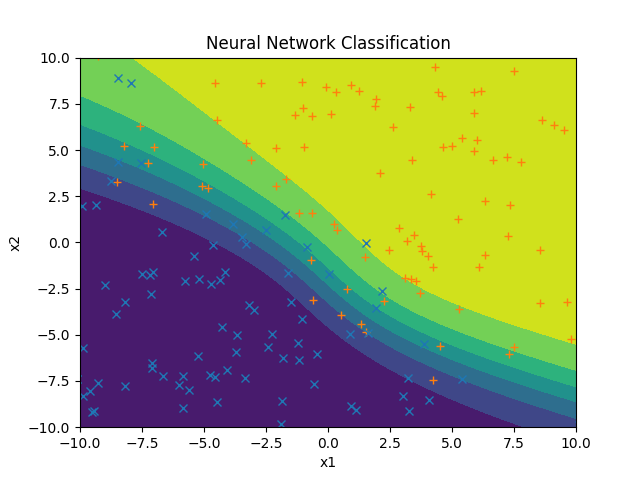
\includegraphics[width=2.8in]{./../code/sgz_result/nn_classification_sgz_l0_002.png}
    \caption{Neural Network Classification on greater than function, when it is using regularization.}
    \label{img:greater_classification_reg}
    \end{center}
\end{figure}

The Neural Network performed well on \textit{xor} function. On the graphs represented by the images from Image \ref{img:xor_cost_reg} to Image \ref{img:xor_classification_reg}. It is also possible to see that in this case, it also heaped much less overfit leading to a much softer image on the graph represented by the Image \ref{img:xor_classification_reg}.

\begin{figure}
  \begin{center}
  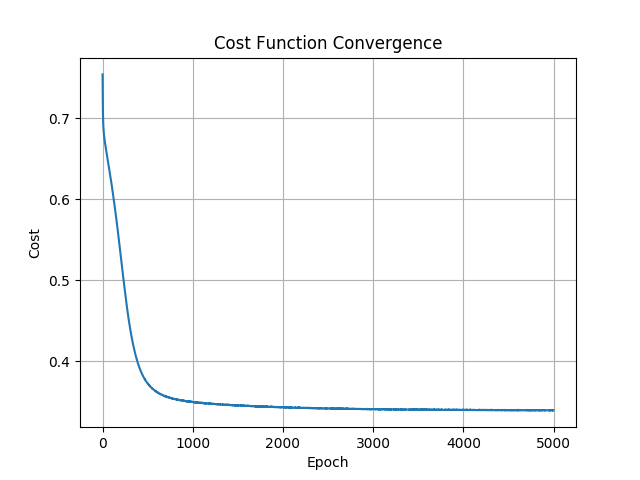
\includegraphics[width=2.8in]{./../code/xor_result/convergence_xor_l0_002.png}
  \caption{Convergence of cost function on xor function test case, when it is using regularization.}
  \label{img:xor_cost_reg}
  \end{center}
\end{figure}

\begin{figure}
    \begin{center}
    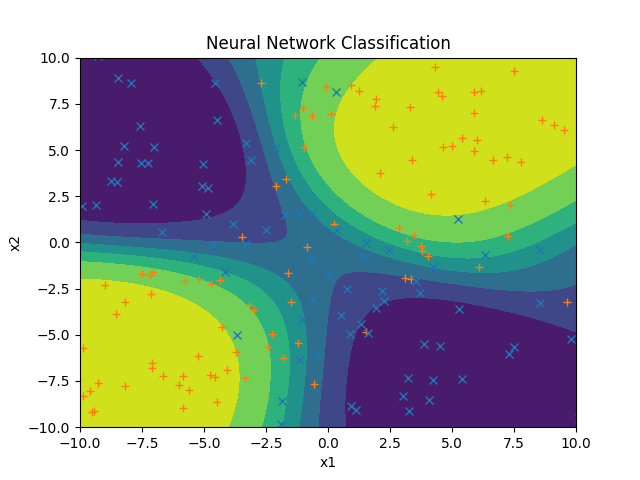
\includegraphics[width=2.8in]{./../code/xor_result/nn_classification_xor_l0_002.png}
    \caption{Neural Network Classification on xor function, when it is using regularization.}
    \label{img:xor_classification_reg}
    \end{center}
\end{figure}

\subsection{Keras' Neural Network Analysis in Imitation Learning}

In order to do the Imitation Learning, it was used the Code \ref{code:imitation} implementation.

It was made using Keras, not using regularization, and using mean squared error.

The result of this Neural Network on the robot movement can be seen on the graphs from Image \ref{img:right_ankle_pitch} to Image \ref{img:right_knee_pitch}.

\begin{figure}
  \begin{center}
  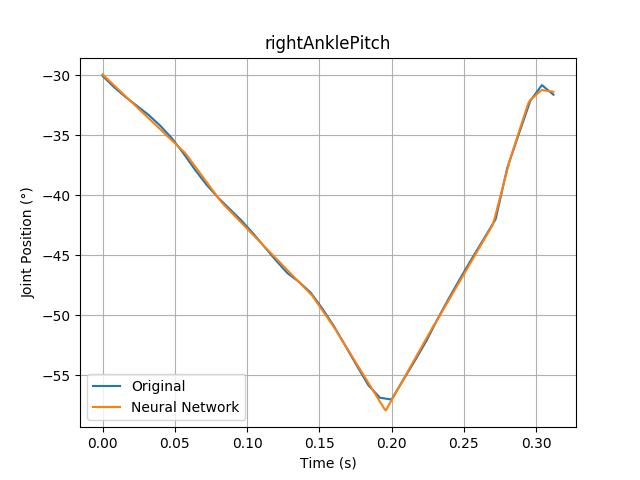
\includegraphics[width=2.8in]{./../code/imitation_learning_result/rightAnklePitch.png}
  \caption{Neural Network's movement imitation of robot's right ankle pitch}
  \label{img:right_ankle_pitch}
  \end{center}
\end{figure}

\begin{figure}
  \begin{center}
  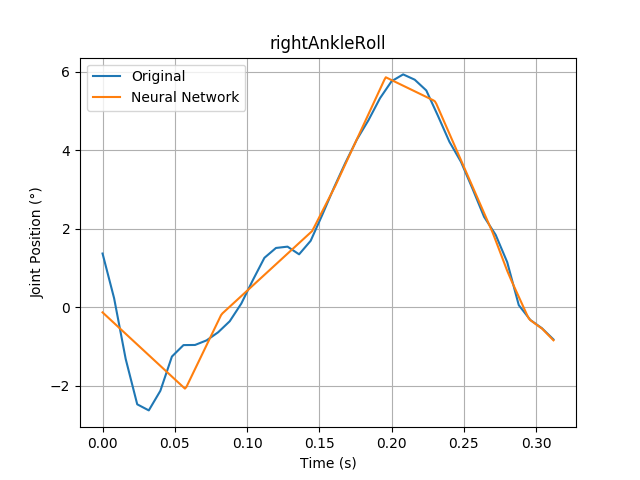
\includegraphics[width=2.8in]{./../code/imitation_learning_result/rightAnkleRoll.png}
  \caption{Neural Network's movement imitation of robot's right ankle roll}
  \label{img:right_ankle_roll}
  \end{center}
\end{figure}

\begin{figure}
  \begin{center}
  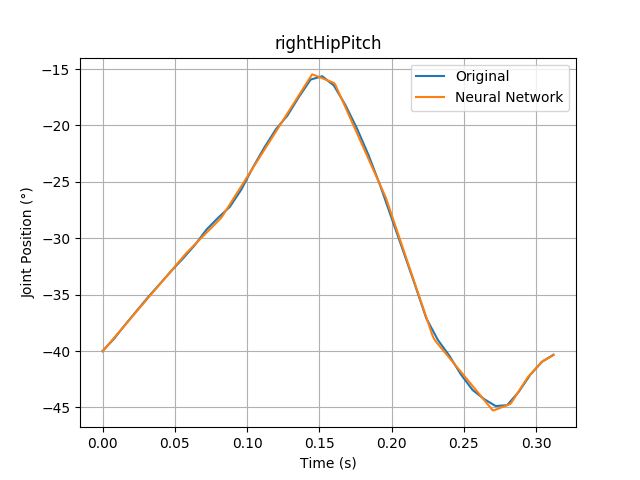
\includegraphics[width=2.8in]{./../code/imitation_learning_result/rightHipPitch.png}
  \caption{Neural Network's movement imitation of robot's right Hip pitch}
  \label{img:right_hip_pitch}
  \end{center}
\end{figure}

\begin{figure}
  \begin{center}
  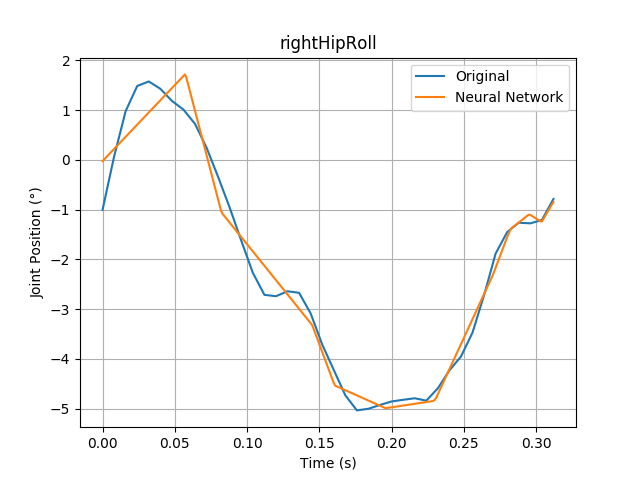
\includegraphics[width=2.8in]{./../code/imitation_learning_result/rightHipRoll.png}
  \caption{Neural Network's movement imitation of robot's right hip roll}
  \label{img:right_hip_roll}
  \end{center}
\end{figure}

\begin{figure}
  \begin{center}
  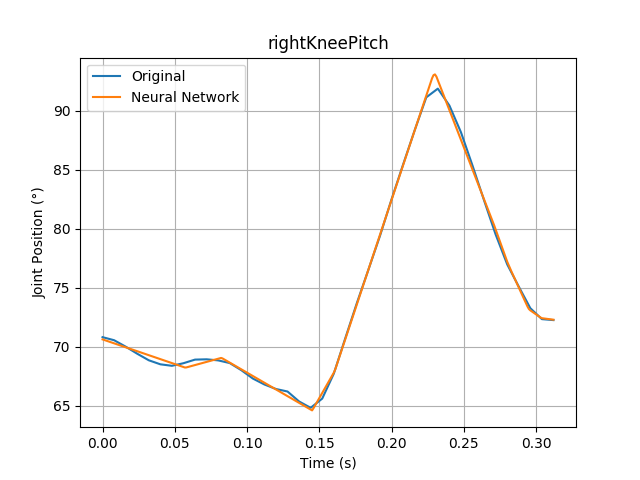
\includegraphics[width=2.8in]{./../code/imitation_learning_result/rightKneePitch.png}
  \caption{Neural Network's movement imitation of robot's right Knee pitch}
  \label{img:right_knee_pitch}
  \end{center}
\end{figure}

\section {Conclusion}

It was clear, therefore, that the Keras' Neural Network worked as expected. Both test cases (greater than function and xor function) the Neural Network worked as well, with a much better result with regularization, because without regularization the results were overfitted.

For the Imitation Learning with Keras, the results were good in some cases and very precise in most some cases.

\vfill
\end{document}
